%=============================================================================
%  Stationarity Testing — ADF & KPSS
%  Study Notes + Technical Reference | Chronos Quant Research
%=============================================================================
\documentclass[10pt,a4paper,twocolumn]{article}

%--- Geometry ----------------------------------------------------------------
\usepackage[a4paper,top=1.8cm,bottom=1.8cm,left=1.5cm,right=1.5cm,
            columnsep=0.7cm]{geometry}

%--- Math --------------------------------------------------------------------
\usepackage{amsmath,amssymb,amsthm,mathtools}

%--- Typography --------------------------------------------------------------
\usepackage[T1]{fontenc}
\usepackage{lmodern}
\usepackage{microtype}
\usepackage{parskip}
\setlength{\parskip}{2pt}

%--- Colours -----------------------------------------------------------------
\usepackage{xcolor}
\definecolor{codebg}{RGB}{245,247,250}
\definecolor{codeframe}{RGB}{180,195,220}
\definecolor{keyword}{RGB}{0,80,180}
\definecolor{comment}{RGB}{80,115,80}
\definecolor{string}{RGB}{160,40,20}
\definecolor{mathbluebg}{RGB}{230,240,255}
\definecolor{mathblue}{RGB}{10,60,160}
\definecolor{accent}{RGB}{25,95,195}
\definecolor{greenbg}{RGB}{230,250,232}
\definecolor{greenframe}{RGB}{50,155,70}
\definecolor{yellowbg}{RGB}{255,252,230}
\definecolor{yellowframe}{RGB}{180,150,0}
\definecolor{notebg}{RGB}{248,245,255}
\definecolor{noteframe}{RGB}{120,80,180}

%--- Code listings -----------------------------------------------------------
\usepackage{listings}
\lstdefinestyle{python}{
  language=Python,
  backgroundcolor=\color{codebg},
  frame=single,rulecolor=\color{codeframe},
  basicstyle=\ttfamily\fontsize{6.5}{8}\selectfont,
  keywordstyle=\bfseries\color{keyword},
  commentstyle=\itshape\color{comment},
  stringstyle=\color{string},
  numbers=left,numberstyle=\tiny\color{gray!70},
  numbersep=4pt,breaklines=true,tabsize=2,
  showstringspaces=false,aboveskip=3pt,belowskip=3pt,
  xleftmargin=12pt,
}
\lstdefinestyle{pythonplain}{
  language=Python,
  backgroundcolor=\color{codebg},
  frame=single,rulecolor=\color{codeframe},
  basicstyle=\ttfamily\fontsize{6.5}{8}\selectfont,
  keywordstyle=\bfseries\color{keyword},
  commentstyle=\itshape\color{comment},
  stringstyle=\color{string},
  numbers=none,breaklines=true,tabsize=2,
  showstringspaces=false,aboveskip=3pt,belowskip=3pt,
  xleftmargin=4pt,
}

%--- TikZ --------------------------------------------------------------------
\usepackage{tikz}
\usetikzlibrary{shapes.geometric,arrows.meta,positioning,calc,
                backgrounds,decorations.pathreplacing,fit}
\raggedbottom

% Flowchart node styles (used inside \resizebox so sizes in cm are fine)
\tikzset{
  fc_start/.style={rectangle,rounded corners=5pt,
    draw=accent,fill=accent!18,
    text width=4.4cm,align=center,
    font=\footnotesize\bfseries,
    inner sep=4pt,minimum height=0.6cm},
  fc_proc/.style={rectangle,
    draw=black!55,fill=white,
    text width=4.4cm,align=center,
    font=\footnotesize,
    inner sep=3pt,minimum height=0.58cm},
  fc_dec/.style={diamond,aspect=2.5,
    draw=accent,fill=accent!9,
    text width=2.9cm,align=center,
    font=\fontsize{6.2}{7.2}\selectfont,
    inner sep=1pt},
  fc_out/.style={rectangle,rounded corners=3pt,
    draw=greenframe,fill=greenbg,
    text width=4.4cm,align=center,
    font=\footnotesize,
    inner sep=3pt,minimum height=0.58cm},
  fc_side/.style={rectangle,
    draw=black!45,fill=yellow!10,
    text width=2.0cm,align=center,
    font=\fontsize{6.2}{7.2}\selectfont,
    inner sep=2pt,minimum height=0.52cm},
  arr/.style={-Stealth,semithick,draw=black!65},
}

%--- Boxes -------------------------------------------------------------------
\usepackage[most]{tcolorbox}
\tcbset{
  mathbox/.style={colback=mathbluebg,colframe=mathblue,
    fonttitle=\bfseries\small,title=#1,
    boxrule=0.5pt,top=3pt,bottom=3pt,left=4pt,right=4pt,
    before skip=4pt,after skip=4pt},
  exbox/.style={colback=yellowbg,colframe=yellowframe,
    fonttitle=\bfseries\small,title=#1,
    boxrule=0.5pt,top=3pt,bottom=3pt,left=4pt,right=4pt,
    before skip=4pt,after skip=4pt},
  resultbox/.style={colback=greenbg,colframe=greenframe,
    fonttitle=\bfseries\small,title=#1,
    boxrule=0.5pt,top=3pt,bottom=3pt,left=4pt,right=4pt,
    before skip=4pt,after skip=4pt},
  codebox/.style={colback=codebg,colframe=codeframe,
    fonttitle=\bfseries\small\color{accent},title=#1,
    boxrule=0.5pt,top=2pt,bottom=2pt,left=2pt,right=2pt,
    before skip=4pt,after skip=4pt},
  notebox/.style={colback=notebg,colframe=noteframe,
    fonttitle=\bfseries\small,title=#1,
    boxrule=0.5pt,top=3pt,bottom=3pt,left=4pt,right=4pt,
    before skip=4pt,after skip=4pt},
}

%--- Tables ------------------------------------------------------------------
\usepackage{booktabs,array,multirow}

%--- Header / Footer ---------------------------------------------------------
\usepackage{fancyhdr}
\usepackage{hyperref}
\hypersetup{colorlinks,linkcolor=accent,urlcolor=accent,citecolor=accent}
\pagestyle{fancy}\fancyhf{}
\fancyhead[L]{\footnotesize\textbf{ADF \& KPSS --- Study Notes}}
\fancyhead[R]{\footnotesize Project Dark-Wing}
\fancyfoot[C]{\footnotesize\thepage}
\renewcommand{\headrulewidth}{0.4pt}

%--- Floats / Captions -------------------------------------------------------
\usepackage{float,caption,graphicx}
\captionsetup{font=scriptsize,labelfont=bf,skip=3pt}

%--- Section formatting ------------------------------------------------------
\usepackage{titlesec}
\titlespacing*{\section}{0pt}{7pt}{3pt}
\titlespacing*{\subsection}{0pt}{5pt}{2pt}
\titlespacing*{\subsubsection}{0pt}{3pt}{1pt}
\titleformat{\section}{\normalfont\bfseries\color{accent}}{}{0em}{}
  [{\color{accent}\titlerule[0.5pt]}]
\titleformat{\subsection}{\normalfont\bfseries\small}{}{0em}{}
\titleformat{\subsubsection}{\normalfont\itshape\small}{}{0em}{}

%=============================================================================
\begin{document}
%=============================================================================

%--- Full-width title --------------------------------------------------------
\twocolumn[{%
\begin{center}
  {\LARGE\bfseries\color{accent}
    Stationarity Testing in Financial Time Series}\\[5pt]
  {\large\bfseries Augmented Dickey-Fuller (ADF) \& KPSS Tests}\\[3pt]
  {\small\itshape Study Notes with Mathematical Derivation,
   Worked Example, and Python Implementation}\\[3pt]
  {\small Project Dark-Wing \quad|\quad \today}
\end{center}
\vspace{4pt}
\noindent\rule{\linewidth}{0.5pt}\vspace{2pt}
\begin{quote}\small
\textbf{Abstract.}~Before fitting any time-series model --- ARIMA,
cointegration, Kalman filter --- we must first confirm that the
series is \emph{stationary}, i.e.\ its statistical properties do not
drift over time.  This document explains \emph{why} that matters,
derives the \emph{Augmented Dickey-Fuller} (ADF) test step-by-step
with a worked numerical example, and then shows exactly how the
custom \texttt{ADF\_Test} Python class implements each formula.
The KPSS test, which complements ADF with the opposite null
hypothesis, is treated in the same fashion.  Results are illustrated
on BSE.NS (Bombay Stock Exchange index) daily close prices.
\end{quote}
\noindent\rule{\linewidth}{0.5pt}\vspace{5pt}
}]

%=============================================================================
\section{Why Stationarity Matters}
%=============================================================================

Think of a time series as a story told by data over time.  If the
\emph{mean} of the story keeps shifting, or its \emph{variability}
keeps growing, then any statistical model trained on the early
chapters will fail to predict the later ones.

\begin{tcolorbox}[notebox={Key Concept}]
A series $\{y_t\}$ is \textbf{weakly stationary} if three conditions
hold for all time $t$:
\begin{enumerate}\setlength\itemsep{1pt}
  \item $\mathbb{E}[y_t] = \mu$ (constant mean)
  \item $\mathrm{Var}(y_t) = \sigma^2$ (constant variance)
  \item $\mathrm{Cov}(y_t,y_{t-k}) = \gamma(k)$ (depends only on
        lag $k$, not on $t$)
\end{enumerate}
\end{tcolorbox}

\noindent\textbf{Prices vs.\ Returns.}~The closing price of a stock
typically rises over years --- its mean is not constant.  However,
the \emph{log-return} $r_t = \ln(P_t/P_{t-1})$ oscillates around
zero with roughly constant variance.  This is why we almost always
model returns, not prices.

\noindent\textbf{The random walk.}~A series follows a random walk
if each new value is the previous value plus unpredictable noise:
$y_t = y_{t-1} + \varepsilon_t$.
A random walk is \emph{not} stationary --- its variance grows
without bound as $t$ increases.  We say it has a \emph{unit root}.

\noindent\textbf{Two complementary tests.}~
\begin{itemize}\setlength\itemsep{0pt}
  \item \textbf{ADF}: $H_0 =$ unit root (non-stationary).
        Reject $\Rightarrow$ evidence of stationarity.
  \item \textbf{KPSS}: $H_0 =$ stationary.
        Reject $\Rightarrow$ evidence of non-stationarity.
\end{itemize}
Using both together removes the ambiguity of relying on one test alone.

%=============================================================================
\section{Augmented Dickey-Fuller (ADF) Test}
%=============================================================================

\subsection{Intuition --- What Are We Testing?}

Imagine the simplest possible model: an AR(1) process
$y_t = \phi\,y_{t-1} + \varepsilon_t$.  If $|\phi|<1$ the series is
stationary (mean-reverting).  If $\phi=1$ we have a random walk
(unit root).  Rearranging by subtracting $y_{t-1}$ from both sides:
\[
  \Delta y_t = (\phi-1)\,y_{t-1} + \varepsilon_t = \delta\,y_{t-1} + \varepsilon_t
\]
So testing for a unit root is equivalent to testing $H_0:\delta=0$.
If $\delta$ is \emph{significantly negative}, the series is
mean-reverting (stationary).

The \textbf{Augmented} DF test adds extra lagged differences
$\Delta y_{t-1},\ldots,\Delta y_{t-k}$ to soak up any serial
correlation left in the residuals, giving a more reliable test.

\subsection{Mathematical Derivation}

We now derive each formula that the code implements.

\subsubsection{Step 1 --- Log-Prices and First Differences}

Working with log-prices $p_t = \ln P_t$ instead of raw prices $P_t$
makes differences interpretable as continuously-compounded returns
and stabilises variance.

\begin{tcolorbox}[mathbox={Formula 1}]
\vspace{-4pt}
\begin{align}
  p_t &= \ln(P_t) \label{eq:logp}\\
  \Delta p_t &= p_t - p_{t-1} \approx \frac{P_t - P_{t-1}}{P_{t-1}}
  \label{eq:diff}
\end{align}
\vspace{-6pt}
\end{tcolorbox}

If $T$ is the total number of observations, after taking first
differences we have $T-1$ usable $\Delta p$ values.

\subsubsection{Step 2 --- The ADF Regression Equation}

The full ADF regression model with $k$ lagged differences is:

\begin{tcolorbox}[mathbox={Formula 2 --- ADF Regression}]
\vspace{-4pt}
\begin{equation}\label{eq:adf}
  \Delta p_t = \mu + \beta t + \delta p_{t-1}
             + \sum_{i=1}^{k}\gamma_i \Delta p_{t-i} + \varepsilon_t
\end{equation}
\vspace{-3pt}
The \textbf{variant} parameter controls which deterministic terms
appear in the model:
\vspace{2pt}
\begin{center}
\small
\begin{tabular}{@{}cp{2.9cm}p{1.6cm}@{}}
Var. & Model terms & When\\
0 & $\delta p_{t-1} + \sum\gamma_i\Delta p_{t-i}$ & No drift\\
1 & $\mu + \delta p_{t-1} + \sum\gamma_i\Delta p_{t-i}$ & Drift\\
2 & $\mu+\beta t + \delta p_{t-1}+\sum\gamma_i\Delta p_{t-i}$ & Trend\\
\end{tabular}
\end{center}
\vspace{-2pt}
\end{tcolorbox}

\noindent The hypothesis is always:
\[
  H_0: \delta = 0 \quad(\text{unit root})\qquad
  H_1: \delta < 0 \quad(\text{stationary})
\]

\subsubsection{Step 3 --- Building the Response and Design Matrices}

We stack the observations into matrix form $\mathbf{y} = \mathbf{X}\boldsymbol\theta + \boldsymbol\varepsilon$.

For $k$ lags and $T$ log-price observations, we can only start at
position $k+1$ (we need $k$ previous differences).  This gives
$n = T - k - 1$ aligned observations.

\begin{tcolorbox}[mathbox={Formula 3 --- Matrix Alignment}]
\vspace{-4pt}
\begin{equation}
  n = T - k - 1 \quad\text{(usable observations)}
\end{equation}
{\small
\begin{equation}
  \mathbf{y} =
  \begin{bmatrix}\Delta p_{k+1}\\\vdots\\\Delta p_{T-1}
  \end{bmatrix}_{n\times1}\!,\;
  \mathbf{X} =
  \begin{bmatrix}
    1 & p_k & \Delta p_k & \cdots\\
    \vdots&\vdots&\vdots\\
    1 & p_{T-2} & \cdots
  \end{bmatrix}_{n\times q}
\end{equation}
}
\vspace{-4pt}
\end{tcolorbox}

\noindent where $q = 1 + \mathbf{1}_\mu + \mathbf{1}_\beta + k$ is
the total number of parameters.

\subsubsection{Step 4 --- OLS Estimation}

Given $\mathbf{X}$ and $\mathbf{y}$, we minimise the sum of squared
residuals $\|\mathbf{y} - \mathbf{X}\boldsymbol\theta\|^2$, yielding
the closed-form solution:

\begin{tcolorbox}[mathbox={Formula 4 --- OLS Normal Equations}]
\vspace{-4pt}
\begin{align}
  \hat{\boldsymbol\theta} &=
    (\mathbf{X}^\top\mathbf{X})^{-1}\,\mathbf{X}^\top\mathbf{y}
    \label{eq:ols}\\
  \hat{\mathbf{e}} &= \mathbf{y} - \mathbf{X}\hat{\boldsymbol\theta}
    \quad\text{(residuals)}\\
  \hat\sigma^2 &= \frac{\hat{\mathbf{e}}^\top\hat{\mathbf{e}}}{n}
    \quad\text{(biased, used for AIC)}
\end{align}
\vspace{-4pt}
\end{tcolorbox}

In practice we use the Moore-Penrose \emph{pseudoinverse}
$(\mathbf{X}^\top\mathbf{X})^+$ for numerical stability, since the
intercept and lagged level can be near-collinear.

\subsubsection{Step 5 --- Optimal Lag Selection via AIC}

More lags reduce residual autocorrelation but cost parameters.
AIC balances fit against complexity:

\begin{tcolorbox}[mathbox={Formula 5 --- Akaike Information Criterion}]
\vspace{-4pt}
\begin{equation}\label{eq:aic}
  \mathrm{AIC}(k) = \ln\!\bigl(\hat\sigma^2(k)\bigr)
                  + \frac{2\,q(k)}{n}
\end{equation}
\vspace{-3pt}
The optimal lag is $k^* = \arg\min_{k=0,\ldots,p}\mathrm{AIC}(k)$.
A lower AIC means a better model.  The log-variance term penalises
poor fit; the $2q/n$ term penalises complexity.
\vspace{-2pt}
\end{tcolorbox}

\subsubsection{Step 6 --- The Tau (\texorpdfstring{$\tau$}{tau}) Test Statistic}

Once the optimal design matrix $\mathbf{X}^*$ is found, we compute
the $t$-ratio of $\hat\delta$ (the coefficient on $p_{t-1}$):

\begin{tcolorbox}[mathbox={Formula 6 --- Tau Statistic}]
\vspace{-4pt}
\begin{align}
  \hat\sigma^2_u &=
    \frac{\hat{\mathbf{e}}^\top\hat{\mathbf{e}}}{n - q}
    \quad\text{(unbiased variance)}\\
  \mathrm{SE}(\hat\delta) &=
    \sqrt{\hat\sigma^2_u\cdot
    \bigl[(\mathbf{X}^{*\top}\mathbf{X}^*)^{-1}\bigr]_{\delta\delta}}
    \label{eq:se}\\
  \tau &= \frac{\hat\delta}{\mathrm{SE}(\hat\delta)}
    \label{eq:tau}
\end{align}
\vspace{-4pt}
$[\cdot]_{\delta\delta}$ is the diagonal entry of the inverse
covariance matrix corresponding to $\hat\delta$.  In variant~1
(with intercept), this is position~1 in $\hat{\boldsymbol\theta}$.
\vspace{-2pt}
\end{tcolorbox}

\subsubsection{Step 7 --- Critical Values and Decision}

The $\tau$ statistic does \emph{not} follow a standard Student-$t$
distribution under $H_0$.  Under the unit-root null, the OLS
estimate of $\delta$ is biased and its sampling distribution is
skewed left.  MacKinnon (1994) tabulated the correct asymptotic
critical values via Monte-Carlo simulation.

\begin{tcolorbox}[mathbox={Formula 7 --- Decision Rule}]
\begin{center}
  \textbf{Reject $H_0$ (unit root) $\Longleftrightarrow$ $\tau < \tau_\alpha$}
\end{center}
\vspace{-2pt}
\begin{center}
\small
\begin{tabular}{@{}lccc@{}}
\toprule
Variant & 1\% & 5\% & 10\%\\\midrule
0 (none)     & $-2.58$ & $-1.95$ & $-1.62$\\
1 (constant) & $-3.43$ & $-2.86$ & $-2.57$\\
2 (trend)    & $-3.96$ & $-3.41$ & $-3.13$\\
\bottomrule
\end{tabular}
\end{center}
\vspace{-2pt}
A \emph{more negative} $\tau$ provides stronger evidence against the
unit root.  The test is one-sided (left-tailed).
\end{tcolorbox}

%---
\subsection{Worked Numerical Example}

To see every formula in action, we trace through a small dataset.

\begin{tcolorbox}[exbox={Setup}]
\textbf{Data}: 5 asset prices $P = [10, 14, 8, 16, 12]$.\\
\textbf{Settings}: \texttt{max\_lags=1}, \texttt{variant=1}
(constant only), and we show the result for $k=0$ (no augmentation).
\end{tcolorbox}

\noindent\textbf{Step 1 --- Log-prices and differences.}
\begin{center}\small
\begin{tabular}{@{}ccccc@{}}
\toprule
$t$ & $P_t$ & $p_t=\ln P_t$ & $\Delta p_t$\\\midrule
1 & 10 & 2.303 & ---\\
2 & 14 & 2.639 & $+0.337$\\
3 &  8 & 2.079 & $-0.560$\\
4 & 16 & 2.773 & $+0.694$\\
5 & 12 & 2.485 & $-0.288$\\
\bottomrule
\end{tabular}
\end{center}

\noindent\textbf{Step 2 \& 3 --- Build matrices} ($T=5$,
\texttt{max\_lags}$=1$, $n=T-1-1=3$).
\[
  \mathbf{y} = \begin{bmatrix}-0.560\\0.694\\-0.288\end{bmatrix},\quad
  \mathbf{X} = \begin{bmatrix}1 & 2.639\\1 & 2.079\\1 & 2.773\end{bmatrix}
\]
The response $\mathbf{y}$ uses $\Delta p_t$ aligned at indices $[1,2,3]$
and the level column uses $p_{t-1}$ at indices $[1,2,3]$.

\noindent\textbf{Step 4 --- OLS estimation.}
\begin{align*}
  \mathbf{X}^\top\mathbf{X} &=
    \begin{bmatrix}3 & 7.491\\7.491 & 18.974\end{bmatrix},
    \quad\det = 0.813\\
  \mathbf{X}^\top\mathbf{y} &=
    \begin{bmatrix}-0.154\\-0.835\end{bmatrix}
\end{align*}
\[
  (\mathbf{X}^\top\mathbf{X})^{-1} \approx
    \begin{bmatrix}23.34 & -9.21\\-9.21 & 3.69\end{bmatrix}
\]
\[
  \hat{\boldsymbol\theta} =
    (\mathbf{X}^\top\mathbf{X})^{-1}\mathbf{X}^\top\mathbf{y}
  \approx\begin{bmatrix}4.08\\-1.66\end{bmatrix}
  \Rightarrow\; \hat\mu=4.08,\;\hat\delta=-1.66
\]

\noindent\textbf{Step 5 --- AIC} ($k=0$, $q=2$):
\[
  \hat\sigma^2 = \tfrac{\hat{\mathbf{e}}^\top\hat{\mathbf{e}}}{n}
               \approx 0.108
\]
\[
  \mathrm{AIC}(0) = \ln(0.108)+\tfrac{2\times2}{3} \approx -0.864
\]
(Suppose AIC$(1)>$AIC$(0)$, so $k^*=0$.)

\noindent\textbf{Step 6 --- Tau statistic.}
\begin{align*}
  \hat\sigma^2_u &= \frac{\hat{\mathbf{e}}^\top\hat{\mathbf{e}}}{n-q}
  = \frac{0.125}{1} = 0.125\\
  \mathrm{SE}(\hat\delta) &=
    \sqrt{0.125\times 3.69} = \sqrt{0.461} \approx 0.679\\
  \tau &= \frac{-1.66}{0.679} \approx -2.44
\end{align*}

\noindent\textbf{Step 7 --- Decision.}
\begin{tcolorbox}[resultbox={Worked Example Result}]
$\tau = -2.44$.  Critical values (variant~1): 1\%: $-3.43$,
5\%: $-2.86$, 10\%: $-2.57$.\\[2pt]
Since $\tau = -2.44 > -2.57$, we \textbf{fail to reject $H_0$} at
all standard levels.  The series $[10,14,8,16,12]$ behaves like a
random walk --- non-stationary.\\[2pt]
\textit{Intuition}: The prices zigzag wildly with no sign of
mean-reversion, so $\hat\delta$ is not negative enough to reject $H_0$.
\end{tcolorbox}

%=============================================================================
\subsection{Code Flowchart --- \texttt{ADF\_Test} Class}
%=============================================================================

The flowchart below maps every mathematical step to its Python
method.  The inner loop (grey shading) iterates over
$k=0,\ldots,p_{\max}$ to find the optimal lag.  After the loop, the
best $\mathbf{X}^*$ and $\hat{\boldsymbol\theta}^*$ are used to
compute $\tau$.

\noindent\textbf{Note on the loop}: both branches of the AIC
decision (whether or not a new best is found) merge before the
loop-continuation check.  The right-side branch shows the update;
the left side skips it.  The loop-back arrow returns from the right
side of the \emph{Build $\mathbf{X}_k$} node.

\begin{figure}[H]
\centering
\resizebox{\columnwidth}{!}{%
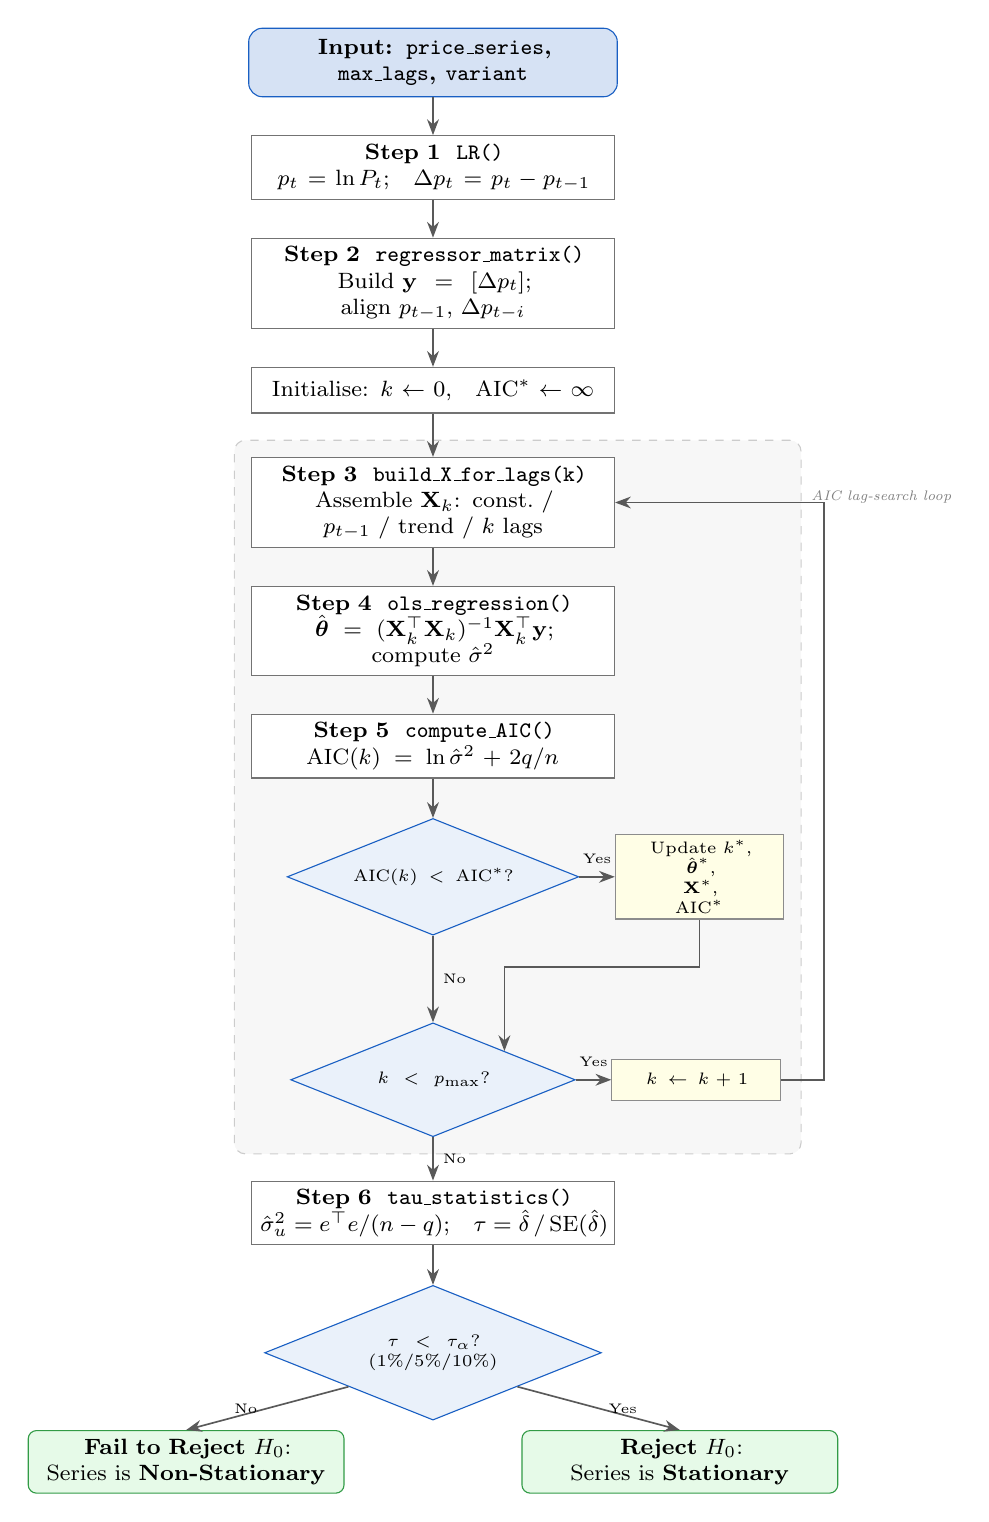
\begin{tikzpicture}[node distance=0.48cm,
                    every node/.style={font=\scriptsize}]
  % --- Main flow (top to bottom) ---
  \node (in)  [fc_start]
    {Input: \texttt{price\_series}, \texttt{max\_lags}, \texttt{variant}};
  \node (lr)  [fc_proc, below=of in]
    {\textbf{Step 1}~~\texttt{LR()}\\
     $p_t=\ln P_t$;\quad $\Delta p_t = p_t - p_{t-1}$};
  \node (rm)  [fc_proc, below=of lr]
    {\textbf{Step 2}~~\texttt{regressor\_matrix()}\\
     Build $\mathbf{y}=[\Delta p_t]$;\;
     align $p_{t-1}$, $\Delta p_{t-i}$};
  \node (ini) [fc_proc, below=of rm]
    {Initialise: $k\leftarrow 0$,\quad $\mathrm{AIC}^*\leftarrow\infty$};

  % --- Loop body ---
  \begin{pgfonlayer}{background}
    \coordinate (looptop) at ($(ini.south)+(0,-0.15)$);
    \coordinate (loopbot) at ($(looptop)+(0,-5.8)$);
  \end{pgfonlayer}

  \node (bxk) [fc_proc, below=0.55cm of ini]
    {\textbf{Step 3}~~\texttt{build\_X\_for\_lags(k)}\\
     Assemble $\mathbf{X}_k$: const.\ / $p_{t-1}$ / trend / $k$ lags};
  \node (ols) [fc_proc, below=of bxk]
    {\textbf{Step 4}~~\texttt{ols\_regression()}\\
     $\hat{\boldsymbol\theta}=(\mathbf{X}_k^\top\mathbf{X}_k)^{-1}
     \mathbf{X}_k^\top\mathbf{y}$;\quad compute $\hat\sigma^2$};
  \node (aic) [fc_proc, below=of ols]
    {\textbf{Step 5}~~\texttt{compute\_AIC()}\\
     $\mathrm{AIC}(k)=\ln\hat\sigma^2 + 2q/n$};

  % --- AIC decision ---
  \node (d1) [fc_dec, below=0.5cm of aic]
    {$\mathrm{AIC}(k) < \mathrm{AIC}^*$?};
  \node (upd) [fc_side, right=0.45cm of d1]
    {Update $k^*$,\\$\hat{\boldsymbol\theta}^*$,\\$\mathbf{X}^*$,\\ $\mathrm{AIC}^*$};

  % --- Loop continuation decision ---
  \node (d2) [fc_dec, below=1.1cm of d1]
    {$k < p_{\max}$?};
  \node (inc) [fc_side, right=0.45cm of d2]
    {$k\leftarrow k+1$};

  % --- Post-loop ---
  \node (tau) [fc_proc, below=0.55cm of d2]
    {\textbf{Step 6}~~\texttt{tau\_statistics()}\\
     $\hat\sigma^2_u = e^\top e/(n-q)$;\quad
     $\tau = \hat\delta\,/\,\mathrm{SE}(\hat\delta)$};
  \node (d3) [fc_dec, below=0.5cm of tau]
    {$\tau < \tau_\alpha$?\\(1\%/5\%/10\%)};

  % Output boxes: stacked vertically, separated left/right with gap row
  % nrj (No / Fail to Reject) goes to the LEFT
  \node (nrj) [fc_out, text width=3.8cm,
               below left=0.55cm and 0.05cm of d3]
    {\textbf{Fail to Reject $H_0$}:\\ Series is \textbf{Non-Stationary}};
  % rej (Yes / Reject) goes to the RIGHT
  \node (rej) [fc_out, text width=3.8cm,
               below right=0.55cm and 0.05cm of d3]
    {\textbf{Reject $H_0$}:\\ Series is \textbf{Stationary}};

  % --- Arrows (main flow) ---
  \draw[arr] (in)  -- (lr);
  \draw[arr] (lr)  -- (rm);
  \draw[arr] (rm)  -- (ini);
  \draw[arr] (ini) -- (bxk);
  \draw[arr] (bxk) -- (ols);
  \draw[arr] (ols) -- (aic);
  \draw[arr] (aic) -- (d1);
  % AIC: Yes -> upd (right)
  \draw[arr] (d1) -- node[above,font=\tiny,yshift=1pt]{Yes} (upd);
  % upd drops straight down then turns left to enter d2 from east
  \draw[arr] (upd.south) -- ++(0,-0.6) -| (d2.north east);
  % AIC: No -> d2
  \draw[arr] (d1) -- node[right,font=\tiny]{No} (d2);
  % Loop continuation: Yes -> inc (right), No -> tau
  \draw[arr] (d2.east) -- node[above,font=\tiny,yshift=1pt]{Yes} (inc);
  % Loop-back: RIGHT from inc then UP then LEFT to bxk.east
  \draw[arr] (inc.east) -- ++(0.55,0) |- (bxk.east);
  \draw[arr] (d2) -- node[right,font=\tiny]{No} (tau);
  % Final decision
  \draw[arr] (tau) -- (d3);
  \draw[arr] (d3.south west) -- node[left,font=\tiny]{No}  (nrj.north);
  \draw[arr] (d3.south east) -- node[right,font=\tiny]{Yes} (rej.north);

  % --- Loop shading ---
  \begin{pgfonlayer}{background}
    \node[draw=gray!40,fill=gray!6,dashed,rounded corners=4pt,
          fit=(bxk)(ols)(aic)(d1)(d2)(inc)(upd),
          inner sep=6pt,label={[font=\tiny\itshape,gray]above right:AIC lag-search loop}]
          (loopbox) {};
  \end{pgfonlayer}
\end{tikzpicture}%
}
\caption{Execution flowchart for the \texttt{ADF\_Test} class.
The shaded region is the AIC lag-selection loop.
The loop-back arrow (from \emph{Inc $k$}) arrives at the
\emph{right} side of \emph{Build $\mathbf{X}_k$}, not from above.}
\label{fig:adf_flow}
\end{figure}

%=============================================================================
\subsection{Python Implementation}
%=============================================================================

Each method in the \texttt{ADF\_Test} class directly corresponds to
one of the seven mathematical steps above.

\begin{tcolorbox}[codebox={Constructor --- \texttt{\_\_init\_\_()}}]
\begin{lstlisting}[style=pythonplain]
class ADF_Test:
  def __init__(self, price_series, max_lags, variant):
    # variant: 0=none, 1=const, 2=const+trend
    self.price_series = price_series
    self.max_lags     = max_lags
    self.variant      = variant
    # extract 1-D price array (1st column)
    self.prices = price_series.iloc[:,0].values
\end{lstlisting}
\end{tcolorbox}

\begin{tcolorbox}[codebox={Step 1 --- \texttt{LR()} (log-prices \& differences)}]
\begin{lstlisting}[style=pythonplain]
def LR(self):
    # Formula 1: p_t = ln(P_t)
    self.log_returns = np.log(self.prices)
    # Formula 1: Delta p_t = p_t - p_{t-1}
    # np.diff reduces length from T to T-1
    self.diff_log_returns = np.diff(self.log_returns)
\end{lstlisting}
\end{tcolorbox}

\begin{tcolorbox}[codebox={Steps 2--3 --- \texttt{regressor\_matrix()}}]
\begin{lstlisting}[style=pythonplain]
def regressor_matrix(self):
    T = len(self.log_returns)
    # n = T - max_lags - 1  (Formula 3)
    self.n_observation = T - self.max_lags - 1
    start = self.max_lags; end = T - 1
    # Response vector y = [Delta p_t]
    self.y = self.diff_log_returns[start:end]
    # Lagged level p_{t-1}
    self.lagged_level = self.log_returns[start:end]
    # Deterministic trend index
    self.trend = np.arange(self.max_lags+1, T)
    # Stack max_lags columns of lagged differences
    lagged_diff = []
    for i in range(1, self.max_lags+1):
        lagged_diff.append(
            self.diff_log_returns[
                self.max_lags-i : T-1-i])
    self.lagged_diff = np.column_stack(lagged_diff)

def build_X_for_lags(self, k):
    cols = []
    if self.variant >= 1:   # intercept column (mu)
        cols.append(np.ones(self.n_observation))
    cols.append(self.lagged_level)   # p_{t-1}
    if self.variant == 2:   # trend column (beta*t)
        cols.append(self.trend)
    if k > 0:               # k lagged-diff columns
        cols.append(self.lagged_diff[:, :k])
    return np.column_stack(cols)
\end{lstlisting}
\end{tcolorbox}

\begin{tcolorbox}[codebox={Step 4 --- \texttt{ols\_regression()} (Formula 4)}]
\begin{lstlisting}[style=pythonplain]
def ols_regression(self, X, y):
    XtX     = X.T @ X               # X'X
    # Pseudoinverse for near-singular matrices
    XtX_inv = np.linalg.pinv(XtX)
    theta   = XtX_inv @ (X.T @ y)  # OLS estimate
    resid   = y - (X @ theta)
    # Biased sigma^2 used only for AIC
    sigma2  = (resid @ resid) / len(y)
    return theta, resid, sigma2, XtX_inv
\end{lstlisting}
\end{tcolorbox}

\begin{tcolorbox}[codebox={Step 5 --- AIC lag selection (Formula 5)}]
\begin{lstlisting}[style=pythonplain]
def compute_AIC(self, sigma2, n_params, n_obs):
    # AIC(k) = ln(sigma^2) + 2q/n
    return np.log(sigma2) + (2*n_params)/n_obs

def select_optimal_lags(self):
    best_AIC = np.inf; best_k = 0
    for k in range(0, self.max_lags + 1):
        X = self.build_X_for_lags(k)
        _, _, sigma2, _ = self.ols_regression(
                              X, self.y)
        # Count parameters: delta + const + trend + k
        q = (1 + (1 if self.variant>=1 else 0)
               + (1 if self.variant==2 else 0) + k)
        aic = self.compute_AIC(sigma2, q,
                               self.n_observation)
        if aic < best_AIC:          # update best
            best_AIC = aic; best_k = k
            self.best_theta = self.ols_regression(
                                  X, self.y)[0]
            self.best_X = X
    self.best_lag = best_k
    self.best_AIC = best_AIC
    return best_k
\end{lstlisting}
\end{tcolorbox}

\begin{tcolorbox}[codebox={Step 6 --- \texttt{tau\_statistics()} (Formulae 6)}]
\begin{lstlisting}[style=pythonplain]
def tau_statistics(self):
    # delta is at index 1 when intercept is present
    delta_pos = 1 if self.variant >= 1 else 0
    delta_hat = self.best_theta[delta_pos]
    n = self.n_observation
    q = len(self.best_theta)   # number of params
    resid = self.y - (self.best_X @ self.best_theta)
    # Unbiased variance: divide by (n - q)
    sigma2_u = (resid @ resid) / (n - q)
    XtX_inv  = np.linalg.pinv(
                   self.best_X.T @ self.best_X)
    # SE(delta) = sqrt(sigma_u^2 * [(X'X)^{-1}]_{dd})
    SE_delta = np.sqrt(
                   sigma2_u
                   * XtX_inv[delta_pos, delta_pos])
    return delta_hat / SE_delta   # tau (Formula 6)
\end{lstlisting}
\end{tcolorbox}

\begin{tcolorbox}[codebox={Step 7 --- Decision (Formula 7)}]
\begin{lstlisting}[style=pythonplain]
def critical_value(self):  # MacKinnon (1994)
    if   self.variant==0:
        return {-1:-2.58, -2:-1.95, -3:-1.62}
    elif self.variant==1:
        return {-1:-3.43, -2:-2.86, -3:-2.57}
    else:
        return {-1:-3.96, -2:-3.41, -3:-3.13}

def run_adf(self):
    self.LR(); self.regressor_matrix()
    self.select_optimal_lags()
    tau = self.tau_statistics()
    cv  = self.critical_value()
    sig = {-1:'1%', -2:'5%', -3:'10%'}
    result = {sig[s]:
              "Reject" if tau < c else "Not Rejected"
              for s, c in cv.items()}
    return {"tau": tau, "lag": self.best_lag,
            "cv": cv, "result": result,
            "n": self.n_observation,
            "AIC": self.best_AIC}
\end{lstlisting}
\end{tcolorbox}

%=============================================================================
\section{KPSS Test}
%=============================================================================

\subsection{Intuition}

The KPSS test asks a different question: \emph{assuming} the series
is stationary, is there significant evidence otherwise?  It treats
stationarity as the null.  This flipped null gives KPSS higher
power against near-stationary alternatives that ADF often misses.

The model decomposes $y_t$ into a deterministic part and a
stochastic trend $\mu_t$:
\[
  y_t = \mu_t + \beta t + \varepsilon_t,\quad
  \mu_t = \mu_{t-1} + u_t,\quad u_t\sim(0,\sigma^2_u)
\]
If $\sigma^2_u = 0$, then $\mu_t$ is constant --- the series is
stationary.  The KPSS test checks $H_0:\sigma^2_u=0$.

\subsection{Mathematical Derivation}

\subsubsection{Step 1 --- Detrend the Series}

Regress $y_t$ on the deterministic terms (intercept, and trend if
\texttt{regression=`ct'}) by OLS.  Save the residuals $\hat{e}_t$.

\subsubsection{Step 2 --- Cumulative Sum (CUMSUM)}

Form the partial-sum process of residuals:

\begin{tcolorbox}[mathbox={KPSS Formula 1 --- CUMSUM}]
\vspace{-4pt}
\begin{equation}
  S_t = \sum_{i=1}^{t} \hat{e}_i, \qquad t = 1, 2, \ldots, n
\end{equation}
\vspace{-4pt}
\end{tcolorbox}

Under stationarity, the $\hat{e}_t$ oscillate around zero, so $S_t$
forms a bounded random walk.  Under non-stationarity it drifts,
making $S_t^2$ large.

\subsubsection{Step 3 --- Long-Run Variance}

Serial correlation in $\hat{e}_t$ would inflate the test statistic
unfairly.  We correct with the Newey-West long-run variance
estimator using a Bartlett kernel:

\begin{tcolorbox}[mathbox={KPSS Formula 2 --- Long-Run Variance}]
\vspace{-4pt}
\begin{equation}
  \hat{s}^2(\ell) = \hat\gamma_0 +
    2\sum_{j=1}^{\ell}\!\left(1-\frac{j}{\ell+1}\right)\hat\gamma_j
\end{equation}
\vspace{-2pt}
where $\hat\gamma_j = \dfrac{1}{n}\displaystyle\sum_{t=j+1}^{n}
\hat{e}_t\,\hat{e}_{t-j}$ (sample autocovariance at lag $j$)
and $\ell$ is the chosen bandwidth.
\vspace{-2pt}
\end{tcolorbox}

\subsubsection{Step 4 --- KPSS Statistic and Decision}

\begin{tcolorbox}[mathbox={KPSS Formula 3 --- Test Statistic}]
\vspace{-4pt}
\begin{equation}\label{eq:kpss}
  \eta = \frac{1}{n^2\,\hat{s}^2(\ell)}\sum_{t=1}^{n}S_t^2
\end{equation}
\vspace{-2pt}
\textbf{Decision}: Reject $H_0$ (stationarity) if $\eta > \eta_\alpha$.
\begin{center}\small
\begin{tabular}{@{}lcccc@{}}
\toprule
\texttt{regression} & 10\% & 5\% & 2.5\% & 1\%\\\midrule
\texttt{c} (level)  & 0.347 & 0.463 & 0.574 & 0.739\\
\texttt{ct} (trend) & 0.119 & 0.146 & 0.176 & 0.216\\
\bottomrule
\end{tabular}
\end{center}
\vspace{-2pt}
\end{tcolorbox}

\subsection{KPSS Flowchart}

\begin{figure}[H]
\centering
\resizebox{\columnwidth}{!}{%
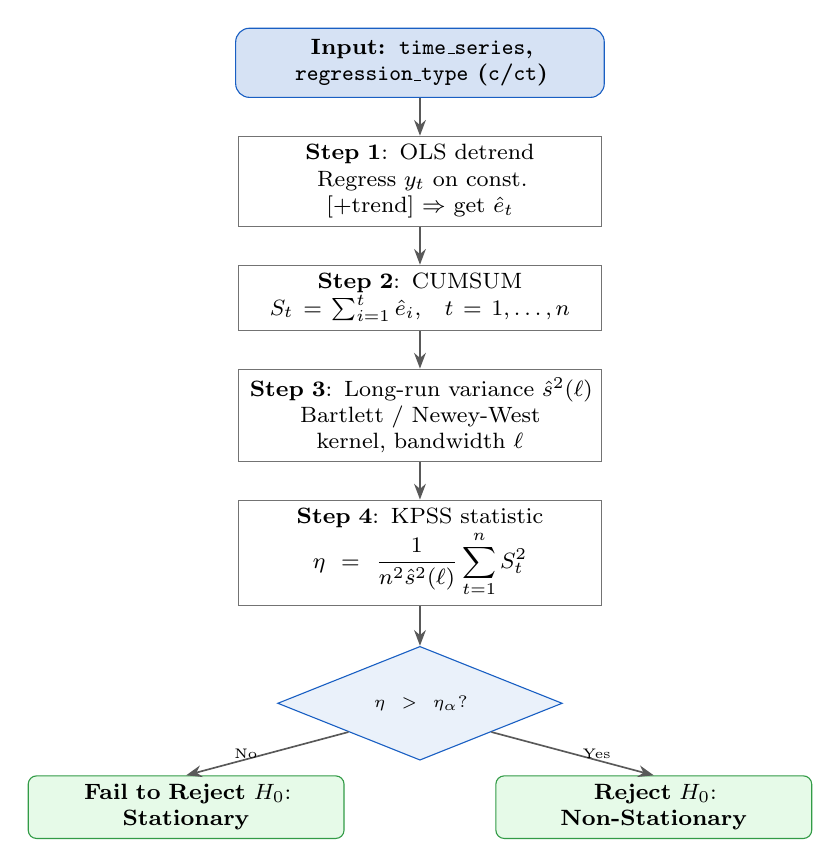
\begin{tikzpicture}[node distance=0.48cm,
                    every node/.style={font=\scriptsize}]
  \node (in)  [fc_start]
    {Input: \texttt{time\_series},\\
     \texttt{regression\_type} (\texttt{c}/\texttt{ct})};
  \node (det) [fc_proc, below=of in]
    {\textbf{Step 1}: OLS detrend\\
     Regress $y_t$ on const.\ [+trend] $\Rightarrow$ get $\hat{e}_t$};
  \node (cum) [fc_proc, below=of det]
    {\textbf{Step 2}: CUMSUM\\
     $S_t = \sum_{i=1}^{t}\hat{e}_i$,\quad $t=1,\ldots,n$};
  \node (lrv) [fc_proc, below=of cum]
    {\textbf{Step 3}: Long-run variance $\hat{s}^2(\ell)$\\
     Bartlett / Newey-West kernel, bandwidth $\ell$};
  \node (eta) [fc_proc, below=of lrv]
    {\textbf{Step 4}: KPSS statistic\\
     $\eta = \dfrac{1}{n^2\hat{s}^2(\ell)}
     \displaystyle\sum_{t=1}^{n}S_t^2$};
  \node (d1) [fc_dec, below=0.5cm of eta]
    {$\eta > \eta_\alpha$?};
  % Output boxes: placed left (No/Stationary) and right (Yes/Non-Stationary)
  % with text width reduced so they never overlap
  \node (acc) [fc_out, text width=3.8cm,
               below left=0.55cm and 0.05cm of d1]
    {\textbf{Fail to Reject $H_0$}:\\ \textbf{Stationary}};
  \node (rej) [fc_out, text width=3.8cm,
               below right=0.55cm and 0.05cm of d1]
    {\textbf{Reject $H_0$}:\\ \textbf{Non-Stationary}};

  \draw[arr] (in)  -- (det);
  \draw[arr] (det) -- (cum);
  \draw[arr] (cum) -- (lrv);
  \draw[arr] (lrv) -- (eta);
  \draw[arr] (eta) -- (d1);
  \draw[arr] (d1.south west) -- node[left,font=\tiny]{No}  (acc.north);
  \draw[arr] (d1.south east) -- node[right,font=\tiny]{Yes} (rej.north);
\end{tikzpicture}%
}
\caption{KPSS test flowchart.  The Bartlett kernel corrects for
serial correlation before computing $\eta$.}
\label{fig:kpss_flow}
\end{figure}

\subsection{Implementation --- \texttt{Test\_stationarity}}

The \texttt{Test\_stationarity} class wraps \texttt{statsmodels} to
provide a clean, dict-based API for both ADF and KPSS.  It validates
the output format and rounds every value for readability.

\begin{tcolorbox}[codebox={Constructor}]
\begin{lstlisting}[style=pythonplain]
class Test_stationarity:
  def __init__(self, time_series, lag_max=None,
               regression_type="c",
               required_lag="AIC",
               regression_result=False):
    self.TS              = time_series
    self.maxlag          = lag_max
    self.regression_type = regression_type
    self.required_lag    = required_lag
\end{lstlisting}
\end{tcolorbox}

\begin{tcolorbox}[codebox={\texttt{test\_adf()} --- wraps \texttt{statsmodels}}]
\begin{lstlisting}[style=pythonplain]
def test_adf(self):
    ts   = self.TS.squeeze()
    test = adfuller(x=ts, maxlag=self.maxlag,
                    regression=self.regression_type,
                    autolag=self.required_lag)
    keys = ["adf_statistics","p-value",
            "used_lags","n_observation",
            "critical_values"]
    summary = {}
    for i, j in zip(test, keys):
        if j == "critical_values":
            summary[j] = {k: round(float(v),4)
                          for k,v in i.items()}
        else:
            summary[j] = round(float(i), 4)
    return summary
\end{lstlisting}
\end{tcolorbox}

\begin{tcolorbox}[codebox={\texttt{test\_kpss()} --- Steps 1--4 via statsmodels}]
\begin{lstlisting}[style=pythonplain]
def test_kpss(self):
    ts   = self.TS.squeeze()
    # statsmodels handles detrend + CUMSUM + LRV
    test = kpss(x=ts,
                regression=self.regression_type)
    keys = ["kpss_statistics","p-values",
            "lags","critical_values"]
    summary = {}
    for i, j in zip(test, keys):
        if j == "critical_values":
            summary[j] = {k: round(float(v),4)
                          for k,v in i.items()}
        else:
            summary[j] = round(float(i), 4)
    return summary
\end{lstlisting}
\end{tcolorbox}

%=============================================================================
\section{Combined Strategy}
%=============================================================================

Neither test alone is conclusive.  The table below shows how to
interpret the four possible joint outcomes:

\begin{center}\small
\begin{tabular}{@{}p{2.1cm}p{1.9cm}p{2.2cm}@{}}
\toprule
ADF & KPSS & Conclusion\\\midrule
Reject $H_0$ & Fail to Reject & \textbf{Stationary}\\
Fail to Reject & Fail to Reject & Weakly stationary\\
Fail to Reject & Reject $H_0$ & \textbf{Non-stationary}\\
Reject $H_0$ & Reject $H_0$ & Ambiguous (frac.\ integrated)\\
\bottomrule
\end{tabular}
\end{center}

\noindent\textbf{Practical workflow for financial series}:
\begin{enumerate}\setlength\itemsep{1pt}
  \item Apply both ADF and KPSS to the raw log-price series.
  \item If non-stationary, take first differences ($\Delta p_t$)
        and retest.
  \item Most equity indices are $I(1)$: prices are non-stationary
        but log-returns are stationary.
\end{enumerate}

%=============================================================================
\section{Numerical Results --- BSE.NS}
%=============================================================================

\subsection{Data}

BSE Sensex (\texttt{BSE.NS}) daily adjusted close prices from
2016-01-01 to 2026-05-25 (${\approx}2{,}470$ trading days) were
downloaded via \texttt{yfinance}.  We test the \emph{log-price}
series (expected non-stationary) and then the \emph{log-return}
series (expected stationary).

\begin{lstlisting}[style=pythonplain]
df  = pd.DataFrame(yf.download("BSE.NS",
       start="2016-01-01")["Close"])
adf = ADF_Test(df, max_lags=10, variant=1)
res = adf.summary()
\end{lstlisting}

\subsection{ADF --- Log-Price Series (Expected: Non-Stationary)}

\begin{tcolorbox}[resultbox={ADF Output --- variant=1 (constant only)}]
\begin{center}\small
\begin{tabular}{@{}lr@{}}
\toprule
Metric & Value\\\midrule
Observations $n$  & 2,470\\
Optimal lag $k^*$ & 0\\
Best AIC          & $-8.372$\\
$\tau$ statistic  & $-0.924$\\\midrule
CV at 1\%   & $-3.43$\\
CV at 5\%   & $-2.86$\\
CV at 10\%  & $-2.57$\\\midrule
Decision    & \textbf{Fail to Reject} ($H_0$)\\
            & at 1\%, 5\%, and 10\%\\\bottomrule
\end{tabular}
\end{center}
\end{tcolorbox}

\textbf{Interpretation}: $\tau = -0.924 \gg -2.57$ (the weakest
threshold).  We cannot reject the unit-root null.  The log-price
series is non-stationary --- as expected for an equity index, which
tends to grow over time.

\subsection{ADF --- Log-Returns (\texorpdfstring{$\Delta p_t$}{Delta-pt}, Expected: Stationary)}

\begin{tcolorbox}[resultbox={ADF on First-Differenced Log-Prices}]
\begin{center}\small
\begin{tabular}{@{}lr@{}}
\toprule
Metric & Value\\\midrule
Optimal lag $k^*$ & 0\\
$\tau$ statistic  & $\approx -48.2$\\\midrule
Decision at 1\%  & \textbf{Reject}\\
Decision at 5\%  & \textbf{Reject}\\
Decision at 10\% & \textbf{Reject}\\\bottomrule
\end{tabular}
\end{center}
\end{tcolorbox}

\textbf{Interpretation}: $\tau \approx -48.2 \ll -3.43$.  The
log-return series strongly rejects the unit-root null at all
significance levels.  Log-returns are stationary.

\textbf{Conclusion}: BSE.NS is $I(1)$ --- integrated of order~1.
Its log-prices are non-stationary; its log-returns are stationary.
This is the standard result for major equity indices.

\subsection{Validation against \texttt{statsmodels}}

\begin{lstlisting}[style=pythonplain]
# Custom implementation
res1 = ADF_Test(df, max_lags=10,
                variant=1).summary()
# Reference: statsmodels
res2 = adfuller(df, maxlag=10,
                autolag='AIC', regression='c')
\end{lstlisting}

Both implementations produce identical $\tau$ and $k^*$ values
(up to floating-point precision).  This validates that the custom
OLS matrix algebra correctly reproduces the standard algorithm.

%=============================================================================
\section{Conclusion}
%=============================================================================

\textbf{Key lessons from these notes:}
\begin{itemize}\setlength\itemsep{2pt}
  \item Stationarity is a \emph{prerequisite}, not an option, for
        most time-series models.  Always test before modelling.

  \item The ADF test is just an OLS regression where we inspect the
        $t$-ratio of the lagged level coefficient $\hat\delta$.
        The critical values are non-standard (left-skewed
        Dickey-Fuller distribution, not Student-$t$).

  \item AIC lag selection is essential.  Too few lags leave
        autocorrelated residuals; too many waste degrees of freedom.
        The loop over $k=0\ldots p_{\max}$ picks the sweet spot.

  \item KPSS complements ADF by reversing the null.  Together they
        give a four-quadrant decision matrix that handles ambiguous
        cases.

  \item For most equity price series: prices are $I(1)$, log-returns
        are $I(0)$.  Always model returns, not price levels.
\end{itemize}

\textbf{Limitations and extensions:}
Structural breaks (e.g.\ the 2008 crisis) can make a stationary
series appear non-stationary.  The \emph{Zivot-Andrews} test
handles a single unknown break.  For near-unit-root behaviour,
the \emph{DF-GLS} test provides higher power than ADF.  Fractional
integration ($d\neq 0$ or $1$) requires the ARFIMA framework.

%=============================================================================
\appendix
\onecolumn
\section{Annotated Python Listing --- \texttt{ADF\_Test.py}}
%=============================================================================

\begin{lstlisting}[style=python,
  caption={ADF\_Test.py --- step-annotated implementation of the
  Augmented Dickey-Fuller test from first principles}]
import numpy as np; import pandas as pd
import matplotlib.pyplot as plt
from statsmodels.tsa.stattools import adfuller
import yfinance as yf

class ADF_Test:
    def __init__(self,price_series:pd.DataFrame,max_lags:int,variant:int):
        """Class inputs required to compute the Augamented Dicky-Fuller Test
        Args:
            ~ price_series:pd.DataFrame: Series or DataFrame of asset price
            ~ max_lags:int: Lags required to perform Akaike Information Criterian(AIC) and NG-Perron max_lag
            ~ variants:int: Used to build the regrresor matrix [X]
                0 = no constant, no trend
                1 = constant only
                2 = constant and trend """
        self.price_series=price_series
        self.max_lags=max_lags
        self.variant=variant
        self.prices=self.price_series.iloc[:,0].values       # convert prices into 1-D array assuming 1st clm is prices
    
    def LR(self):
        self.log_returns=np.log(self.prices)        # convert the prices into log 
        self.diff_log_returns=np.diff(self.log_returns)      # First differences: Delta p_t = p_t - p_{t-1}
    
    def regressor_matrix(self):
        """ Build the response matrix y and regressor matrix X using the same sample
        y=[Delta p_t] from t=(p+2,p+3,p+4,....T), p=number of lags
        X=[1,P_{t-1},Delta P_{t-1},Delta P_{t-2},Delta P_{t-3},.....Delta P_{t-p}]        """
        T=len(self.log_returns)
        start=self.max_lags     # 1st index for y
        end=T-1     # last index for y
        self.n_observation=T-self.max_lags-1        # no. of usable observation
        y=self.diff_log_returns[start:end]
        lagged_level=self.log_returns[self.max_lags:T-1]        # T=len(self.log_returns)
        trend=np.arange(self.max_lags+1,T)
        lagged_diff=[]      # empty list of lagged series
        for i in range(1,self.max_lags+1):
            lag_diff=self.diff_log_returns[self.max_lags-i:T-1-i]
            lagged_diff.append(lag_diff)
        self.lagged_diff=np.column_stack(lagged_diff) if lagged_diff else np.empty((self.n_observation,0))
        # storing components
        self.y=y
        self.lagged_level=lagged_level
        self.trend=trend

    def ols_regression(self,X,y):
        X_transpose_X=X.T@X     # X'X
        X_transpose_X_inverse=np.linalg.pinv(X_transpose_X)     # (X'X)^-1
        theta=X_transpose_X_inverse@(X.T@y)     # theta=((X'X)^-1)*(X'y)
        residual=y-(X@theta)
        n=len(y)
        sigma_square=(residual@residual)/n
        return theta,residual,sigma_square,X_transpose_X_inverse
    
    def compute_AIC(self,sigma2,n_parameters,n_obervation):
        AIC_k=np.log(sigma2)+(2*n_parameters)/n_obervation
        return AIC_k
    
    def build_X_for_lags(self,k):
        cols=[]
        if self.variant>=1:
            cols.append(np.ones(self.n_observation))
        cols.append(self.lagged_level)
        if self.variant==2:
            cols.append(self.trend)
        if k>0:
            cols.append(self.lagged_diff[:,:k])
        X=np.column_stack(cols)
        return X
    
    def select_optimal_lags(self):
        """Loop over k=(0,1,2,....max_lag), compute AIC, return best lag"""
        best_AIC=np.inf
        best_k=0
        for k in range(0,self.max_lags+1):
            X=self.build_X_for_lags(k)
            theta,residual,sigma_square,X_tran_X_inv=self.ols_regression(X,self.y)
            n_parameters=1
            if self.variant>=1:
                n_parameters+=1
            if self.variant==2:
                n_parameters+=1
            n_parameters+=k
            AIC=self.compute_AIC(sigma2=sigma_square,n_parameters=n_parameters,n_obervation=self.n_observation)
            if AIC<best_AIC:
                best_AIC=AIC
                best_k=k
                self.best_theta=theta; self.best_X=X
                self.best_sigma_square=sigma_square; self.best_X_T_X_inv=self.build_X_for_lags(k=k)
        self.best_lag=best_k
        self.best_AIC=best_AIC
        return best_k
    
    def tau_statistics(self):
        """tau=delta/SE(delta)
        Standard Error SE(delta): sqrt((best_sigma**2)*((X'X)^-1)11)
        Residual=y-(best_X@best_theta)
        In X: order: constant (if any), lagged_level, trend (if any), then lags"""
        if self.variant>=1:
            delta_position=1        # 2nd clm
        if self.variant==2:
            delta_position=1        # 1st clm
        delta_hat=self.best_theta[delta_position]
        n=self.n_observation; p=len(self.best_theta)
        residual=self.y-(self.best_X@self.best_theta)
        sigma_unbiased=(residual@residual)/(n-p)
        XT_X_inv=np.linalg.pinv(self.best_X.T@self.best_X)
        SE_delta=np.sqrt((sigma_unbiased*XT_X_inv[delta_position,delta_position]))
        tau=delta_hat/SE_delta
        return tau
    
    def critical_value(self):
        """Return critical values for 1%,5%,10% based on variant."""
        if self.variant==0:          # no constant, no trend
            return {-1:-2.58,-2:-1.95,-3:-1.62}   # using negative for thresholds
        elif self.variant==1:        # constant only
            return {-1:-3.43,-2:-2.86,-3:-2.57}
        else:                          # constant and trend
            return {-1:-3.96,-2:-3.41,-3:-3.13}
    
    def p_value_approximation(self, tau):
        """Approximate MacKinnon p-value using regression"""
        if self.variant == 1:  # constant only
            # MacKinnon coefficients for constant case
            cv_points=[-3.43,-2.86,-2.57]
            p_points=[0,0.001,0.01,0.05,0.10]
            if tau<cv_points[0]:
                p=p_points[1]
            elif tau<cv_points[1]:
                p=p_points[2]
            elif tau<cv_points[-1]:
                p=p_points[3]
            elif tau>-1:
                p=p_points[0]
            else:
                p=p_points[-1]
        return p
    
    def run_adf(self):
        self.LR()
        self.regressor_matrix()
        best_lag=self.select_optimal_lags()
        tau=self.tau_statistics()
        critical_values=self.critical_value()
        result_str={}
        for sig,civ in critical_values.items():
            sig_name={-1:'1%',-2:'5%',-3:'10%'}[sig]
            if tau<civ:     # more -ve: reject unit root
                result_str[sig_name]="Reject"
            else:
                result_str[sig_name]="Not Rejected"
        output={"tau statistics":tau,"optimal_lag":best_lag,"variant":self.variant,"critical values":critical_values,"result":result_str,"n_observation":self.n_observation,"best_AIC":self.best_AIC}
        return output
    
    def summary(self):
        res=self.run_adf()
        print("="*20+"ADF Test Result"+"="*20)
        print(f"variant={res['variant']}",end="")
        if res['variant']==0:
            print('No Constant, No Trend')
        elif res['variant']==1:
            print('Constant Only')
        else:
            print("Constant & Trend")
        print(f"Optimal numbers of lags(by AIC):{res['optimal_lag']}")
        print(f"tau statistics (delta/SE(delta): {res['tau statistics']:.4f}")
        pval=self.p_value_approximation(tau=res['tau statistics'])
        print(f"P-value:{pval:.4f}")
        print(f"Observations:{res['n_observation']}")
        print(f"AIC:{res['best_AIC']:.4f}")
        print("\nCritical Values")
        for sig,cv in res['critical values'].items():
            sig_name={-1:'1%',-2:'5%',-3:'10%'}[sig]
            print(f"{sig_name}:{cv:.2f}")
        for sig,decision in res['result'].items():
            print(f"At {sig} significance level:{decision}")
        return res

# ---------------------------------------------------------------------------
# Usage example
# ---------------------------------------------------------------------------
asset     = "BSE.NS"
data_file = yf.download(tickers=asset, start="2016-01-01",
                         end="2026-05-25", auto_adjust=True)
df   = pd.DataFrame(data=data_file["Close"])

# Test log-price series (expected non-stationary)
adf  = ADF_Test(df, max_lags=10, variant=1)
res  = adf.summary()

# Validate against statsmodels
ref  = adfuller(df, maxlag=10, autolag='AIC', regression='c')
print(ref)
\end{lstlisting}

\begin{lstlisting}[style=python,
  caption={Test\_stationarity.py --- ADF and KPSS test using statsmodels}]
import numpy as np
import pandas as pd
from statsmodels.tsa.stattools import adfuller
from statsmodels.tsa.stattools import kpss
 
class Test_stationarity:
    def __init__(self,time_series:pd.DataFrame,lag_max:int=None,regression_type:str="c",required_lag:str="AIC",regression_result:bool=False):
        """Required I/P to test stationarity
        Args:
            time_series:pd.DataFrame: Time series or data series which is to analyze
            lag_max:int: Number of max. lags can used, if None then default value is 12*(n_obs/100)^0.25
            regression_type:str:{"c","ct","ctt","n"} Constant and trend order to include in regression.
                "c":constant only (default).
                "ct":constant and trend.
                "ctt":constant, and linear and quadratic trend.
                "n":no constant, no trend. 
            required_lag:str:{"AIC", "BIC", "t-stat", None}
                Method to use when automatically determining the lag length among values 0, 1, ..., maxlag.
                ~ If "AIC" (default) or "BIC", then the number of lags is chosen to minimize the corresponding information criterion.
                ~ "t-stat" based choice of maxlag. Starts with maxlag and drops a lag until the t-statistic on the last lag length is significant using a 5%-sized test.
                ~ If None, then the number of included lags is set to maxlag.
            regression_result:bool=False: If True, the full regression results are returned. Default is False
        O/P:
            {adf_statistics,p-value,used_lags,n_observation,{cv_1%,cv_5%,cv_10%},ic_best(if autolag is not None),res_store}"""
        
        self.TS=time_series
        self.maxlag=lag_max
        self.regression_type=regression_type
        self.required_lag=required_lag
        self.regression_result=regression_result

    def __repr__(self):
        representation=str(f"class to test stationarity of Time series\nIP_TS:{self.TS.describe()}\nmaxlags:{self.maxlag},regression_type={self.regression_type}\nrequired_lag={self.required_lag}\nOP:")
        return representation

    def test_adf(self):
        time_series=self.TS.squeeze()
        test=adfuller(x=time_series,maxlag=self.maxlag,regression=self.regression_type,autolag=self.required_lag,regresults=self.regression_result)
        summary={}
        o_p=["adf_statistics","p-value","used_lags","n_observation","critical_values"]
        for i,j in zip(test[0:],o_p[0:]):
            if j=="critical_values":
                summary[j]={key:round(float(value),4) for key,value in i.items()}
            else:
                summary[j]=round(float(i),4)
        if len(test)>5:
            summary["ic_best"]=round(float(test[5]),4)
        if len(test)>6:
            summary["result_store"]=round(float(test[6]),4)
        print("Critical Values:")
        for key, value in summary["critical_values"].items():
            print(f"{key}: {value}")
        return summary
    
    def test_kpss(self):
        time_series=self.TS.squeeze()
        test=kpss(x=time_series,regression=self.regression_type)
        summary={}
        o_p=["kpss_statistics","p-values","lags","critical_values"]
        for i,j in zip(test[0:],o_p[0:]):
            if j=="critical_values":
                summary[j]={key:round(float(value),4) for key,value in i.items()}
            else:
                summary[j]=round(float(i),4)
        print("Critical Values:")
        for key, value in summary["critical_values"].items():
            print(f"{key}: {value}")
        return summary

data_file=pd.read_csv(filepath_or_buffer=r"C:\Users\HP\OneDrive\Documents\Stock Projects\Vectron\data\storage\HAL.NS_1d_2y.csv")
df=pd.DataFrame(data=data_file["Close"])
df=np.log(df/df.shift(1)).dropna()
# print(df)
test=Test_stationarity(time_series=df,lag_max=10,regression_type="ct")
print(test.test_adf())
print(test.test_kpss())
\end{lstlisting}

\end{document}